\documentclass[letterpaper,12pt]{article}
\usepackage{tabularx} % extra features for tabular environment
\usepackage{amsmath}  % improve math presentation
\usepackage{graphicx} % takes care of graphic including machinery
\usepackage[margin=1in,letterpaper]{geometry} % decreases margins
\usepackage{cite} % takes care of citations
\usepackage[final]{hyperref} % adds hyper links inside the generated pdf file
\hypersetup{
	colorlinks=true,       % false: boxed links; true: colored links
	linkcolor=blue,        % color of internal links
	citecolor=blue,        % color of links to bibliography
	filecolor=magenta,     % color of file links
	urlcolor=blue         
}
\usepackage[square,numbers]{natbib}

\usepackage[utf8]{inputenc}
\usepackage[TS1,T1]{fontenc}
% \usepackage{fourier, heuristica}
\usepackage{array, booktabs}
\usepackage{graphicx}
\usepackage[x11names,table]{xcolor}
\usepackage{caption}
\usepackage{multicol}
\setlength{\columnsep}{2cm}
\DeclareCaptionFont{blue}{\color{LightSteelBlue3}}

\bibliographystyle{abbrvnat}

\newcommand{\foo}{\color{LightSteelBlue3}\makebox[0pt]{\textbullet}\hskip-0.5pt\vrule width 1pt\hspace{\labelsep}}

\begin{document}

\title{Undergraduate Research Thesis Proposal: Generating Expressive Musical Performance}
\author{Richard Timpson}
\date{\today}
\maketitle

\begin{abstract}
    Recent advances in deep learning and big data processing have led to the development of powerful applications in computer vision, natural language processing (NLP), speech processing, and audio recognition. Related to these fields, especially NLP and speech processing, is the computational study of music and music information retrieval (MIR). This thesis will further work in this area by examining musical expressiveness and its relationship to automatic score performance rendering. Previous work in this area has been limited to small datasets and recurrent neural networks. We propose a study involving state of the art seq-2-seq Transformer based neural network models using a new data corpus that is orders of magnitudes larger than similar datasets. 
\end{abstract}


\section{Introduction}
When the convolutional neural network AlexNet \cite{krizhevsky2012imagenet} won the ImageNet classification competition in 2012 with a significantly lower error rate than other models, it shocked the Machine Learning, Artificial Intelligence, and Computer Science communities as a whole. Since then there has been a continual significant improvement in both machine learning related algorithms and hardware architecture which have led to the rise of “Deep Learning” and powerful applications in several domains including computer vision, speech and audio processing, natural language processing, robotics, bioinformatics, and more \cite{goodfellow2016deep}. 

The computational study of music dates back to the early days of computer science when Lejaren Hiller and Leonard Issacson programmed a computer that would write the first musical score\footnote{\url{https://www.youtube.com/watch?v=n0njBFLQSk8}} produced by an electronic computer in 1957 \cite{sandred2009revisiting}. This has led to the broad study in the intersection of music and computer science which we conceptually divide into two broad categories: analysis and generation. Generative models deal both with the instrumental synthesis of actual sounds and the composition of symbolic music. To draw out an analogy with human-language technologies, musical composition corresponds to language and text generation whereas instrument synthesis corresponds with speech generation. 

Analysis models usually are categorized as work within music information retrieval (MIR) \cite{widmer2016getting} which involves using computers to empirically extract out patterns and information from raw music. The most common task in MIR is Genre or Artist recognition, and is the central focus of musical recommendation systems, with Spotify pushing the state of the art in industry \footnote{\url{https://research.spotify.com}}.

Musical expressiveness is a multi-disciplinary aspect of musical study that includes contributions from musicology, music psychology, and MIR. Generally speaking, it is the study of the relationship between the score of a music composition and a related performance (or performances) produced by a musician \cite{cancino2018computational}. No two performances of the same piece of music are identical (even if they are by the same performer); there is an inherent interpretation of a score in every single musical performance. From a MIR perspective, this poses questions about the extent to which musical expressiveness can be accurately modeled both computationally and mathematically. Some of the current tasks in MIR related to expressiveness include analysis of error in performance \cite{flossmann2010magaloff}, and identifying the style of particular performer over another \cite{grachten2012linear}. 

The focus of this thesis is in the actual generation of expressive performances as opposed to the analysis of a particular performance or performer. There are industry products available that can render performances given a score\footnote{MuseScore is the most popular. \url{https://musescore.com}}, however, they have a mechanical aspect to them. This is akin to the early days of speech synthesis which produced robotic voices without prosodic cues. An expressive performance system would be able to take in a musical score as its input and produce a performance that should sound as if it was produced by a human. In that sense, the proposed model may fit better as a generation model as opposed to analytical, but can realistically be seen as existing within the intersection of both paradigms, as is shown in Figure \ref{musical-models}

\begin{figure}[!htb]
	\center
	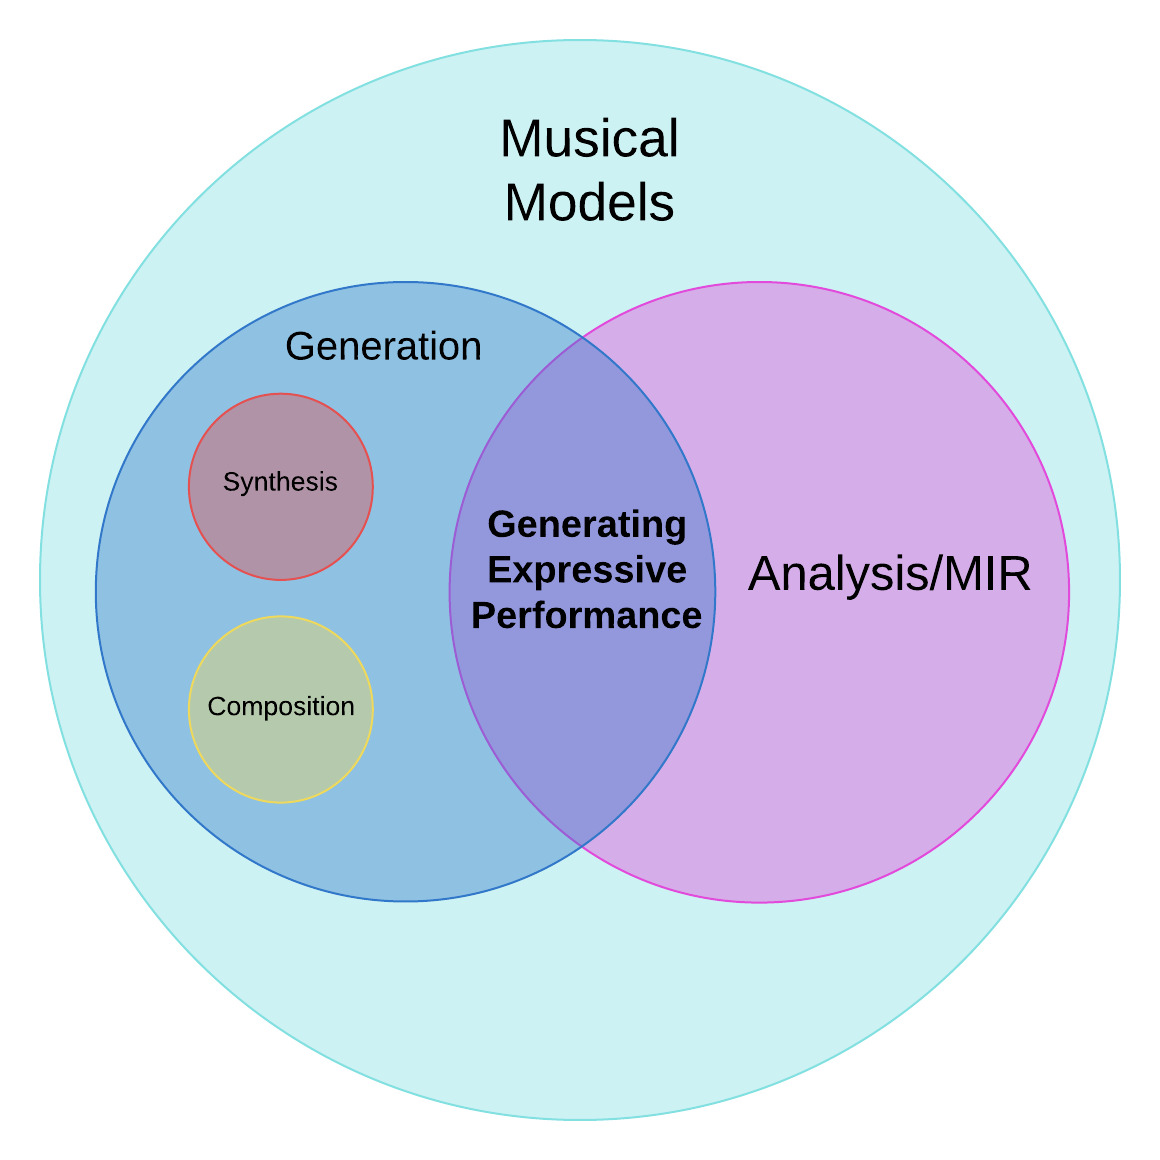
\includegraphics[width=0.6\linewidth]{images/musical-models.png}
	\caption{Musical models broken down by category. Our model sits at the intersection of generation and analysis}
	\label{musical-models}
\end{figure}

\section{Background}
Both music and language are highly sequential, creative in nature, and are embedded within a hierarchical structure of rules that are inherently statistical (music theory for music and grammar for language). Because of this and the fact that NLP receives a larger focus in the research literature, seq-2-seq models that have shown remarkable success in NLP have a natural extension into music and should be considered inside of MIR where applicable. 
\subsection{State of the art in Deep Learning and NLP}

Traditional seq-2-seq models in Deep Learning have centered around Recurrent Neural Networks (RNN) and a common modification as a Long Short Term Memory (LSTM) Neural Network. In recent years there has been a move away from RNN’s towards a model known as a Transformer which relies solely on the use of attention based mechanisms which are better at learning long term structure of sequences \cite{vaswani2017attention}. One of the key ideas behind Transformers is that they do not require an in-order processing of a sequence (unlike RNNs) and are therefore highly parallelizable \cite{devlin2018bert}. This has led to the development of general NLP models trained on massive datasets which can achieve state of the art results on several different NLP tasks \cite{devlin2018bert} \cite{radford2019language}. 

\subsection{Music and Machine Learning}
Much work has already been accomplished in taking a data-driven approach to modeling music, both from the analytical and generative perspective. The previous work done in modeling musical expressiveness has (to our knowledge) been limited to simple linear models \cite{grachten2012linear}, simple probability based models \cite{widmer2009yqx}, and more recently RNNs \cite{chacon2016basis} \cite{jeong2019virtuosonet}. Generative composition models however, have seen the application of Transformers with impressive results \cite{huang2018music}. 

\subsubsection{Modeling Musical Expressiveness}
Widmer \cite{widmer2000potential} introduces the study of music using machine learning in general, and specifically uses modeling musical expressiveness as one of its applications. He splits the model into two representations; one at an individual note level and the other at a musical structure level. His results show that learning at a structural level (a phrase or measure) is better than by individual notes, which indicates that the context of the music plays an important role in the performance. Grachten \cite{grachten2012linear} continues this work by developing the Linear Basis Model (LBM) for modeling musical expressiveness. The LBM takes in annotated music in the form of a symbolic score (as opposed to single notes or an entire phrase as in the previous model), and uses a set of defined linear basis functions to encode elements of the score as features for a simple linear regression model which outputs the correlating expressive parameters (the dynamics or tempo of a note). 

Chacon \cite{chacon2016basis} extends the LBM using a RNN to build the “Basis Mixer,” which is a more robust system given the dynamic nature of RNNs. Jeong \cite{jeong2019virtuosonet} also uses an RNN with hierarchical attention layers to build the virtuosoNet. To our knowledge, virtuosoNet appears to be the most sophisticated model published, and will form the basis for much of the research in this thesis. Samples from the model's performances can be found online\footnote{virtuosoNet playing Chopin Fantasie impromptu (it was absent from the training dataset): \url{https://www.youtube.com/watch?v=BN0ZCBS9q0Y}}. 

\subsubsection{Modeling Musical Generation with Transformers}
Briot \cite{briot2017deep} gives a complete overview of deep learning techniques that have been used for music generation. Perhaps the most important architecture for future work, the Transformer, is missing from his overview, and so we will touch on the work that has happened so far in the area. The Magenta research project\footnote{\url{https://magenta.tensorflow.org/}} is an effort by Google to use machine learning to make music and art. They have created several systems that use Transformers for music generation, most notably one that can create music with long term structure \cite{huang2018music}. 

\subsection{Data}
Given the diverse nature of music and its applications, the musical technology that exists today is inherently multimedia based. There are several different data representations involved with music, from pure symbolic note annotations to audio waves and sound frequencies. For systems that are involved with generating performances, there are generally two key facets for the data modeling to be productive. One is the score of a composition, which represents the symbolic form of the music (commonly known as sheet music). The other is the actual performance of the piece of music rendered by a musician. Scores are typically represented as MusicXML, and performances as MIDI. 

\subsubsection{Scores as MusicXML}
MusicXML is self-descriptive. It uses the commonly known XML format to represent the symbolic form of a musical score. It includes metadata about scores such as the name of the composition, the timing of the piece, and the key signature – as well as detailed information about every individual note including the pitch, timing, and other score annotations related to dynamics. MusicXML was introduced as a potential internet standard for score representations and is often used as a way to import/export compositions between different commercially available software systems. Traditionally, scores were represented according to proprietary protocols specific to industry applications, and MusicXML was introduced to be a bridge between these different applications \cite{good2001musicxml}. 

\subsubsection{Performances as MIDI}
The Musical Instrument Digital Interface (MIDI) is a standard internet protocol for data representation and hardware interfaces for musical instruments\footnote{\url{https://www.midi.org/}}. It encodes both information about the pitch and timing of notes played as well as related expressive parameters of those notes. Most importantly, it encodes the dynamics of a note which is represented as MIDI velocity. It is important to note that MIDI can, in a sense, represent both the score and the performance as it encodes information about which notes are played (score) and how they are played (expression). However, MusicXML is a more rich standard when it comes to score representation as it contains information about every relevant score annotation, and provides information that allows more robust models \cite{grachten2012linear}. 

\section{Modeling}
To our knowledge, there is no existing expressive performance rendering system that makes use of a Transformer based neural network architecture. Given that Transformers have taken over the state of the art in many NLP related tasks and have already seen successful application to music composition generation, the central question this thesis would like to pose is the extent to which Transformers are useful in modeling musical expressiveness and if they can outperform existing expressive performance models according to an established baseline. We will present a formal definition of an expressive performance model, the baseline models that currently exist, and potential new Transformer based model architectures. 

\subsection{Defining Musical Expressiveness}
As has already been mentioned, musical expressiveness is the study of the relationship between the score of a musical composition and a related performance of the composition by a given performer. It includes various aspects of musical parameters, such as tempo, timing, dynamics, intonation, and articulation \cite{cancino2018computational}. The most prevalent expressive parameter in musical performance is dynamics, and relates to how loud or soft a particular note or region of notes is played. When a musical phrase is annotated as forte (meaning loud), it is up to the performer to decide how loud to actually render the phrase, which can possibly depend on a number of other contextual variables such as how loud they are currently playing, the pitch of the note(s) being played \cite{grachten2012linear}, the articulation of a note, and even the current mood of the performer. In this example, a forte marking is part of the symbolic score and its associated expressive parameter, dynamics, is part of the performance (represented in MIDI as velocity). 


\subsection{Expressive Performance Model}
Our goal is to build a model that maps scores to expressive performance. We denote the former as d-dimensional vectors $x$. Let $X = \{x_1, x_2, x_3...x_n\}$ be the sequence of score features that represent an entire composition. Some features that are commonly used to represent the score are pitch, note duration, dynamic markings, and phrasing \cite{cancino2018computational}. We denote the expressive performance features as k-dimensional vector $y$ and a performance sequence $Y = \{y_1, y_2, y_3, ... y_n\}$. Common expressive parameters are dynamics (as MIDI velocity), timing (as note onset deviations), and articulation (as the note duration) \cite{cancino2018computational}. We will explore a family of generative expressive models $U$, which map each element in the score sequence to an associated expressive parameter in the performance sequence, so that $Y = U(X)$. Modeling choices need to be made about the $d$ score features, $k$ performance features, and the generative model $U$ which is to be trained given a dataset of symbolic scores and related performances. The score features are typically derived from MusicXML, and the performance features from MIDI. 

\subsection{Baseline}
One of the main limitations in studying musical expressiveness is the lack of large scale high quality datasets that are publicly available and provide both a score and its related performance information \cite{cancino2018computational}. In \cite{jeong2019virtuosonet}, Jeong contributes a publicly available and relatively new dataset that is 10 times larger than the similar Magaloff Corpus \cite{flossmann2010magaloff} which has been commonly used for similar systems. The dataset makes use of the Yamaha Signature MIDI collection, which provides MIDI files associated with performances from the Yamaha e-Competitions of western classical piano music\footnote{\url{http://www.yamahaden.com/midi-files}}. Along with the MIDI, this dataset also provides the corresponding MusicXML files for every composition as well as a note-level alignment between the MusicXML score and the performance MIDI. Given the easy access and scale of the dataset, it will be used for our research

In \cite{jeong2019virtuosonet} Jeong also provides an overview of the virtuosoNet which contains the output evaluation metrics for predicting the output expressive features for several different model. The implementation of the PyTorch models and experiments that create virtuosoNet are available as an open source repository\footnote{\url{https://github.com/jdasam/virtuosoNet}}. These models are hierarchical attention networks (HAN) which make use of bi-directional LSTMs at different levels of abstraction, beginning at the individual note level and ending at an entire measure level. The hierarchical LSTMs are stitched together using a multi-head attention, and the result is a set of networks that can take in a score as MusicXML and output an expressive performance in MIDI. 

\subsection{Proposed Contributions}
The main contribution of this thesis will be to make use of a Transformer in generating expressive performance, building off of the baseline work already established with the virtuosoNet. The focus for this research will be in answering the question 
	\begin{quote} \textit{Will a Transformer based neural network architecture relying strictly on attention outperform the existing virtuosoNet, which uses a hierarchical attention network and relies on recurrent neural networks?}
	\end{quote}
Because of the recent trend in related state of the art NLP research away from RNNs and towards Transformers, we hypothesize that the answer to this question will be yes. 

In addition to experimenting with the predictive model, we would also like to explore how the feature engineering and data pre-processing affects the performance of the model. Jeong outlines in detail the different input score and output performance features that he uses with the HAN \cite{jeong2018virtuosonet}. Further exploration into additional features for both the score representation and expressive performance may be warranted, with potential for an improvement in the models results. 

Given the need for more high quality data for modeling musical expressiveness and in MIR in general, it may also be worth it to explore gathering additional score and performance data if possible. Jeong provides a strong basis for data gathering and processing, so the addition of more data in the form of MusicXML and MIDI may be trivial. It is also worth mentioning that because Transformers are more parallelizable than RNNs, we also expect to see an improvement in training and inference speeds and can take better advantage of having a larger dataset. 

The possibility for achieving significant results for all of these contributions is yet to be determined and will depend on the difficulty of running the initial experiments. At the very least, we would like to build the Transformer architecture and compare it to virtuosoNet as a baseline – the other goal contributions would be ideal but are not necessary. Listed in order according to priority, the specific goals are: 

\begin{enumerate}
	\item Build Transformer model(s) for expressive performance generation and compare it to the HAN in the virtuosoNet
	\item Explore the possibility of adding additional input/output features and measure their effect on model performance
	\item Gather more score data (MusicXML) and performance data (MIDI) and add it to the data corpus used to train virtuosoNet
\end{enumerate}

\section{Experiment}
Because virtuosoNet is open source it will act as a basis for model development and data processing. The source for virtuosoNet includes all the necessary tools to process data, create both input and output features, build and train models, and use the models to create an expressive performance in MIDI form given a score in MusicXML. The first goal for the experiment will be to reproduce the model and results presented in \cite{jeong2019virtuosonet}. 

With the full end to end system in place, we can then build and implement different Transformer architectures and add them to the existing system pipeline. The next goal will include building a simple Transformer that fits within the existing system and will act as an additional source for model comparison and evaluation. With a basic Transformer in place, we can then add additional complexities (with influences from related models in music generation and NLP language models) to fine tune and identify the best performing model. Once this has happened, we will have met the first goal. 

If the time and resources permit, we can then experiment with additional feature representation and measure its effects on model performance. Finding and adding more data to the corpus would be the last effort of the experiment, and would add more validity to the results and findings. If this happens, we will have met the second and third goals. 

\subsection{Evaluation}
Jeong provides an overview of the evaluation for his baseline and advanced models in \cite{jeong2019virtuosonet}. His model evaluation uses the mean-squared-error (MSE) of several different output expressive parameters from the model. These expressive parameters are tempo, velocity, note onset deviation, articulation, and pedal sustain. For our model evaluation we will use the same metric with the same expressive parameters as our baseline comparison with the goal to improve upon his existing models. 

If the time and resources permit, we may also be adding additional expressive parameters (which are still to be determined) to the model using MSE as our evaluation. Given that all of the code for virtuosoNet is open source, we can also re-build Jeong's existing models and evaluate them on any new expressive features that we find. This will provide a solid basis for comparison and allow for the interpretability of our results. 

\section{Timeline}
The following is a proposed timeline for the remainder of the thesis project, starting from the beginning of the experiment and culminating in the writing and submitting of the thesis paper. 
% https://tex.stackexchange.com/a/196808

\begin{table}[h]
\begin{multicols}{2}
	\renewcommand\arraystretch{1.4}\arrayrulecolor{LightSteelBlue3}
	\captionsetup{singlelinecheck=false, font=blue, labelfont=sc, labelsep=quad}
	\caption{Experiment Timeline}\vskip -1.5ex
	\begin{tabular}{@{\,}r <{\hskip 2pt} !{\foo} >{\raggedright\arraybackslash}p{5cm}}
	\toprule
	\addlinespace[1.5ex]
	Week of 6/29 & Start experiment\\
	Week of 7/13 & Built and reproduced the results from virtuosoNet\\
	Week of 8/1  & Built and implemented baseline Transformer model\\
	Week of 8/24 & Built and implemented advanced Transformer\\
	Week of 9/21 & Added feature engineering and additional data. 
	% If model development is not sufficient for robust results, feature engineering and data gathering should be suspended. 
	\end{tabular}
	\columnbreak
	\renewcommand\arraystretch{1.4}\arrayrulecolor{LightSteelBlue3}
	\captionsetup{singlelinecheck=false, font=blue, labelfont=sc, labelsep=quad}
	\caption{Writing Timeline}\vskip -1.5ex
	\begin{tabular}{@{\,}r <{\hskip 2pt} !{\foo} >{\raggedright\arraybackslash}p{5cm}}
	\toprule
	\addlinespace[1.5ex]
	Week of 9/21 & Start thesis writing\\
	Week of 11/1 & First draft of thesis finished\\
	Date of 11/12 & Give oral presentation (last day of classes)\\
	Date of 11/25 & Finalize and submit thesis (last day of exams)\\
	\end{tabular}
\end{multicols}
\end{table}

\pagebreak
\bibliography{bibliography}

\end{document}